%% Paper 1: how stable is the top of a gridded European heat-wave catalogue
%% when the detector's own settings change? 36 summers, 1991-2026.
%%
%% Needs the AMS LaTeX package version 6. Two files are NOT in this repository
%% and have to be downloaded from the AMS LaTeX submissions page, which refuses
%% automated requests, then placed beside this file:
%%
%%     ametsocV6.cls    the document class
%%     ametsocV6.bst    the bibliography style
%%
%% https://www.ametsoc.org/ams/publications/author-information/latex-author-info/
%%
%% Editorial Manager builds the PDF from the source, so do not upload a PDF of
%% your own. Figure files it receives must carry flat names with no directory
%% path, no underscores and no periods before the extension, which is why the
%% figure macros below expect fig1.pdf and not plots/detection/europe_....pdf.
%%
%% Compile: pdflatex, bibtex, pdflatex, pdflatex.

%% PREVIEW: swap back to ametsocV6 once the AMS files are here.
\documentclass{amsdraft}

\usepackage{amsmath,amsfonts,amssymb,bm}
\usepackage{mathptmx}
\usepackage{newtxtext}
\usepackage{newtxmath}
\usepackage{graphicx}
% Written by paper/write_numbers.py from paper/results/. Do not edit.
\providecommand{\missingnumber}{\textbf{??}}
\newcommand{\AUCFit}{0.76}
\newcommand{\AUCValidate}{0.82}
\newcommand{\BaselineK}{19}
\newcommand{\BaselineKRest}{1}
\newcommand{\BaselineN}{30}
\newcommand{\BaselineNRest}{6}
\newcommand{\BrierClimatology}{0.247}
\newcommand{\BrierValidate}{0.175}
\newcommand{\EdgeK}{18}
\newcommand{\EdgeKRest}{2}
\newcommand{\EdgeN}{33}
\newcommand{\EdgeNRest}{3}
\newcommand{\LeadEvenOdds}{38}
\newcommand{\LeadOhThree}{8}
\newcommand{\LeadTwentySix}{45}
\newcommand{\LeadTwentyTwo}{30}
\newcommand{\LeaderMovedHi}{70}
\newcommand{\LeaderMovedLo}{40}
\newcommand{\LeaderShareMedian}{88}
\newcommand{\MedianDurationOhThree}{5}
\newcommand{\MedianDurationTwentySix}{6}
\newcommand{\MedianDurationTwentyTwo}{5}
\newcommand{\NEventsMedian}{30}
\newcommand{\NEventsOhThree}{34}
\newcommand{\NEventsTwentySix}{38}
\newcommand{\NEventsTwentyTwo}{36}
\newcommand{\NForEightyOhThree}{7}
\newcommand{\NForEightyTwentySix}{7}
\newcommand{\NForEightyTwentyTwo}{5}
\newcommand{\NLeaderAbsorbed}{8}
\newcommand{\NLeaderAgreeAll}{12}
\newcommand{\NLeaderJJA}{16}
\newcommand{\NLeaderMoved}{20}
\newcommand{\NLeaderMovedNorm}{23}
\newcommand{\NLeaderMovedRefBar}{18}
\newcommand{\NLeaderSplit}{0}
\newcommand{\NMovedArea}{9}
\newcommand{\NMovedAreaNorm}{9}
\newcommand{\NMovedAreaRefBar}{9}
\newcommand{\NMovedConnectivity}{2}
\newcommand{\NMovedConnectivityNorm}{2}
\newcommand{\NMovedConnectivityRefBar}{2}
\newcommand{\NMovedDays}{11}
\newcommand{\NMovedDaysNorm}{13}
\newcommand{\NMovedDaysRefBar}{11}
\newcommand{\NMovedGrid}{22}
\newcommand{\NMovedGridNorm}{24}
\newcommand{\NMovedGridRefBar}{21}
\newcommand{\NMovedPercentile}{14}
\newcommand{\NMovedPercentileNorm}{16}
\newcommand{\NMovedPercentileRefBar}{12}
\newcommand{\NMovedRawWindow}{8}
\newcommand{\NMovedRawWindowNorm}{6}
\newcommand{\NMovedRawWindowRefBar}{4}
\newcommand{\NMovedWindow}{4}
\newcommand{\NMovedWindowNorm}{8}
\newcommand{\NMovedWindowRefBar}{3}
\newcommand{\NSummers}{36}
\newcommand{\NTopPairMerged}{11}
\newcommand{\NTopThreeLeft}{18}
\newcommand{\PBaseline}{0.069}
\newcommand{\PCrowding}{0.95}
\newcommand{\PEdge}{1}
\newcommand{\PLead}{0.0074}
\newcommand{\PSeason}{0.31}
\newcommand{\RhoCrowding}{$-$0.01}
\newcommand{\RhoLead}{$-$0.44}
\newcommand{\SeasonK}{7}
\newcommand{\SeasonKRest}{13}
\newcommand{\SeasonN}{16}
\newcommand{\SeasonNRest}{20}
\newcommand{\TopOneShareOhThree}{23}
\newcommand{\TopOneShareTwentySix}{25}
\newcommand{\TopOneShareTwentyTwo}{31}
\newcommand{\TopSixShareOhThree}{78}
\newcommand{\TopSixShareTwentySix}{78}
\newcommand{\TopSixShareTwentyTwo}{87}
\newcommand{\TopThreeShareOhThree}{56}
\newcommand{\TopThreeShareTwentySix}{50}
\newcommand{\TopThreeShareTwentyTwo}{67}


\title{TITLE DEFERRED: written last, from the finished results}

%% AMS designates ONE corresponding author on the title page. The
%% corresponding author in Editorial Manager can be a different person.
\authors{Isaac Adoboe\correspondingauthor{Isaac Adoboe, ieadoboe@mun.ca}
and Elsa Cardoso-Bihlo}

\affiliation{Memorial University of Newfoundland, St. John's,
Newfoundland and Labrador, Canada}

\abstract{ABSTRACT DEFERRED: written last, once the results and conclusions
are settled.}

\begin{document}

\maketitle

%% Optional for a journal article, required for BAMS, at most 120 words.
% \statement
% Significance statement here.

\section{Introduction}
\label{sec:intro}

European summer heat waves are among the most damaging weather extremes the
continent experiences. The summer of 2003 was statistically extremely
unlikely even when the observed warming is taken into account
\citep{Schar2004}, and more than 70\,000 additional deaths occurred during it
\citep{Robine2008}; the summer of 2010, centred on eastern Europe and Russia,
then exceeded 2003 in both amplitude and spatial extent
\citep{Barriopedro2011}; and the summer of 2022 was associated with more than
60\,000 heat-related deaths \citep{Ballester2023}. Over the past four decades,
heat-wave trends over Europe have been three to four times faster than over
the rest of the northern midlatitudes \citep{Rousi2022}.

Deciding which of these events were the most severe is usually the job of a
catalogue. Ranked lists of the most severe European heat waves
\citep{Russo2015,Becker2022,LhotkaKysely2022} and classifications of their
spatial patterns \citep{Stefanon2012} determine which events are studied in
depth, and physical storylines of extreme heat are constructed around a
chosen case \citep{WhittakerDiLuca2026}. Extreme-event attribution starts
from the choice of an event and its definition \citep{Philip2020}, and it is
well established that attribution statements depend on the spatial and
temporal scale at which that event is defined
\citep{Angelil2014,CattiauxRibes2018,Leach2020}; \citet{Cattiaux2024} went on
to propose an objective way of selecting the most extreme temperature events.
Those studies vary the definition of an event once it has been chosen. They
leave open an earlier question: whether the choice of which event to study,
when it is read off the top of a catalogue, is itself stable.

There is no single definition of a heat wave
\citep{PerkinsAlexander2013,Perkins2015}. Indices developed for station
records count hot days at a point \citep{Zhang2011}, whereas a gridded
catalogue must also decide how large a hot region has to be before it
constitutes an event \citep{Stefanon2012,Lhotka2015}. Every such detector has
settings with no physically correct value: the percentile that defines a hot
day, the window over which that percentile is estimated, the minimum
duration and area of an event, and the neighbourhood that joins hot cells
into one object. The frequency, trends and geographic patterns of heat waves
depend strongly on the index adopted \citep{Smith2013}, and the ranking of
historical European events shifts between intensity indices
\citep{Becker2022}. Within event-based detectors, the area threshold,
connectivity and overlap criterion alter heat-wave metrics and their trends
\citep{Zhang2025}, and \citet{Mandonnet2026} ran a 96-member ensemble of a
three-dimensional European detector, varying the percentile, minimum
duration, baseline and connectivity, to evaluate heat-wave indices against
impact records. \citet{BrunnerVoigt2024} showed that pooling a percentile
over a running window without first removing the seasonal cycle raises the
threshold where the seasonal cycle is steep, so that exceedances are
undercounted, most strongly in spring and autumn, and
\citet{Meindl2024} found that the bias also changes the size and duration of
the largest heat waves in climate projections. None of these studies reports
whether the event a catalogue ranks first stays first when the detector's
own settings change, nor what makes a summer's ranking fragile.

This paper asks that question for 36 European summers, 1991--2026, and
uses the answer to build a catalogue whose ranking is stable. We build a
gridded CTX90pct catalogue from ERA5 for each summer under a reference
configuration, rerun it with each setting changed in turn across the range
used in the literature, and record what happens to the leading event: whether
it holds, is overtaken, absorbs another leading event, or breaks up. We then
trace the instability to its sources (the way the threshold window is
pooled, the bar against which each run is scored, and the measure of
severity) and test whether a catalogue built to avoid them keeps its leader:
the seasonal cycle removed before the percentile is taken, European land
only, and events ranked by severity normalized by local variability. For
the instability that remains, we test whether it can be predicted from how
far a summer's leader is ahead, and repeat the experiment for Canada to test
that prediction in a second region. Section~\ref{sec:methods} describes the data, the
detector and the experiment; section~\ref{sec:results} presents the results;
section~\ref{sec:discussion} considers what they imply for building and using catalogues;
and section~\ref{sec:conclusions} summarizes.

\section{Data and methods}
\label{sec:methods}

\subsection{Reanalysis data and domain}
\label{sec:data}

We built the catalogue from daily maximum 2-m temperature in the ERA5
reanalysis \citep{Hersbach2020}, retrieved from the Copernicus Climate Data
Store as the derived daily-statistics product. The European box spans
35--72$^\circ$N and 25$^\circ$W--45$^\circ$E on the native 0.25$^\circ$ grid,
149 latitudes by 281 longitudes. Each summer was retrieved from 1 April to 31
October, so that an event already under way on 1 May, or still running on 30
September, is measured whole; an event enters the catalogue of a summer if at
least one of its days falls between 1 May and 30 September.
%% TODO: state the retrieval date of each 2026 month and whether it is ERA5T;
%% rerun 2026 on final ERA5 before submission.

Ocean cells were removed with a land mask from the 0.1$^\circ$
K\"oppen-Geiger map of \citet{Beck2023}, sampled to the ERA5 grid by nearest
neighbour. Land outside Europe was then removed as well: a cell is kept if
the nearest 0.1$^\circ$ cell lies in a country that Natural Earth assigns to
Europe, or in Cyprus; a coastal land cell whose centre falls outside every
country outline takes the nearest country. The box otherwise reaches North Africa, Anatolia and
the Middle East, which would let events there lead a European catalogue. An
event that reaches the outer ring of the box, or a cell next to excluded
land, is flagged as cut off in space, since its true extent is unknown.

The second region, Canada, spans 41.5--84$^\circ$N and 141--52$^\circ$W and
keeps Canadian land only; it was processed identically.

\subsection{Heat-wave threshold}
\label{sec:index}

The index is CTX90pct \citep{PerkinsAlexander2013}, applied to every land
cell independently. For each cell and calendar day $d$ the threshold
$T_{90}(d,i,j)$ is the 90th percentile of daily maximum temperature over the
1991--2020 baseline, pooling every baseline day within $\pm$7 days of $d$.
Pooled directly, such a window mixes days with different climatological
normals, which widens the sample and biases the percentile where the
seasonal cycle is steep \citep{BrunnerVoigt2024}. We therefore first
subtracted from each baseline day its own normal, a 31-day running mean
across all baseline years, took the percentile of the residuals within the
window, and added the normal of day $d$ back. Calendar days are taken as
day of year.

Each summer inside the baseline was judged against the other 29 years, so
that it never helps set its own threshold; each threshold from 8 April to
24 October then rests on $29 \times 15 = 435$ samples, and those nearer the
ends of the retrieved span on fewer. Summers after 2020 use all 30 years.

\subsection{Detection}
\label{sec:coherence}

A 90th-percentile threshold places about one tenth of all cell-days above it
by construction, so a background of scattered exceedances covers the domain
on any day. Labelling that field directly lets isolated cells bridge
unrelated patches and chain them into one object. The detector therefore
works in four steps, in this order. First, hot cell-days are those above
their threshold, on retained land. Second, within each day hot cells are
grouped into patches under eight-connectivity (four-connectivity in the
6-neighbour runs of section~\ref{sec:sensitivity}), and every patch smaller than
$A_{\min}$ is discarded, with areas from the spherical cell areas
\begin{equation}
A(i) = R^2 \, \Delta\phi \, \Delta\lambda \, \cos\phi_i ,
\label{eq:area}
\end{equation}
$R = 6371.0088$ km. Third, a cell-day is kept only if the cell lay in such a
patch on at least three consecutive days, implemented as a binary opening
along time; persistence is thus counted inside large patches, not on raw hot
days. Fourth, the surviving cell-days are labelled as connected components
in (time, latitude, longitude) \citep{Virtanen2020}, joining each cell to its
eight spatial neighbours on the same day and to itself on the previous and
next day. Because the opening can trim a day's patch, single days of an event
may fall below $A_{\min}$; an event is retained if its largest day reaches it.
The reference uses $A_{\min} = 50\,000$ km$^2$, comparable to the area of
Slovakia.

\subsection{Severity and attributes}
\label{sec:events}

Each event $E$ carries a severity
\begin{equation}
S = \sum_{(t,i,j)\,\in\,E}
    \left[ T_{\max}(t,i,j) - T_{90}(d_t,i,j) \right] A(i) ,
\label{eq:severity}
\end{equation}
in $^\circ$C km$^2$ day, by which the catalogue is ranked. An event scores
highly by being hot, large and long together. Unlike the heat wave magnitude
indices of \citet{Russo2014,Russo2015}, $S$ is not normalized by local
variability, so it weighs regions and months with a wide spread of daily
maxima more heavily; it is closest to the extremity index of
\citet{LhotkaKysely2022}.

Two further rankings are computed for every run. $S_{\mathrm{ref}}$ sums,
over the run's cell-days, the exceedance above the reference threshold,
floored at zero, instead of the run's own, so a stricter percentile changes
which cells count but not how they are scored. $S_{\mathrm{norm}}$ divides
each cell-day's exceedance by the local interquartile range of baseline
daily-maximum anomalies (seasonal cycle removed) in the 15-day reference
window, floored at 0.1$^\circ$C, in the spirit of \citet{Russo2015}. For each event we also recorded its dates,
peak and mean daily areas, highest daily maximum, largest exceedance, peak
day (the day of greatest mean exceedance over the event's cells), the
area-weighted centroid on that
day, and whether it is cut off in time (it touches the first or last day
retrieved) or in space (section~\ref{sec:data}).

\subsection{Sensitivity experiment}
\label{sec:sensitivity}

The reference configuration is the 90th percentile, a 15-day window with the
seasonal cycle removed, $A_{\min} = 50\,000$ km$^2$, a minimum duration of 3
days and 10-neighbour labelling. Each summer was rerun with one setting
changed at a time across the range found in published practice: the
percentile at 90, 92.5, 95 and 97.5; the window at 7, 11, 15, 21 and 31 days;
$A_{\min}$ at 25\,000, 50\,000, 100\,000, 250\,000 and 625\,000 km$^2$, the
last the threshold of \citet{LhotkaKysely2022}; the minimum duration at 3 to
6 days, as in \citet{Mandonnet2026}; and labelling with 6, 10 or 26
neighbours \citep{Zhang2025}. Because percentile and minimum duration are the
settings most likely to move the leader, they were also crossed in a
$4 \times 4$ grid. The 7-, 15- and 31-day windows were rerun once more with
raw pooling, which
measures the bias the reference avoids rather than a defensible choice. We
call the reference configuration ranked by $S_{\mathrm{norm}}$ the recipe: it
removes the seasonal cycle, keeps European land only and normalizes severity,
the three choices section~\ref{sec:results} tests.

\subsection{Matching and outcomes}
\label{sec:matching}

The labelling numbers components in scan order, so no event identifier
survives a change of configuration. Every reference event was matched to the
catalogued event of the other run with which it shares the most cell-days, provided that
event holds at least half of the reference event's cell-days. Matching on
shared cell-days, unlike matching on dates and centroids, cannot mistake a
small event that vanished for one that merged into a large neighbour.

The fate of the reference leader under each run is one of five outcomes. It
\emph{held} if its match still ranks first and no other of the six leading
reference events matched the same object; it was \emph{absorbed} if it still
ranks first but another leading event merged into it, so the case is a
different object; it was \emph{replaced} if its match no longer ranks first;
it \emph{split} if it overlaps two or more events of the run,
none holding half its cell-days; and it \emph{vanished} otherwise, that is,
if none of its cell-days survives in a catalogued event or the only piece
that does holds less than half. A summer's leader is said
to move when, under at least one single change of setting, it was replaced or
vanished. Absorption and splitting are reported separately: they change what
a case study would analyse without changing which event tops the list.

\subsection{Statistics}
\label{sec:stats}

Counts of summers carry 95\% Wilson intervals. Whether a setting moves
leaders more often than chance is judged against a null model in which the
setting only adds symmetric noise to the log severity ratio of the first two
events, Gaussian with a standard deviation equal to that of the changes in
the log ratio that setting value actually produced, over the summers in which
both events were matched; the expected number of moves sums, over summers,
the probability that such noise exceeds that summer's own gap. The lead of a
summer is $1 - S_2/S_1$ in the reference catalogue. Its association with the
number of single changes that move the leader, and that of crowding (pairs
of leading events within three days and $10^\circ$ of each other), are
Spearman rank correlations against that same outcome; crowding counts pairs
among the six leading events whose dates overlap or lie at most three days
apart and whose centroids lie within $10^\circ$, longitude scaled by the
cosine of latitude. Summers whose leader peaks in June to August, summers
inside the baseline and leaders cut off in space are
compared with the rest by Fisher's exact test. A logistic regression of
whether the leader moves on the logarithm of the lead was fitted to the
European summers and evaluated on the Canadian ones by the area under the
ROC curve and the Brier score against a constant forecast of the Canadian
move rate; summers with a lead of zero are left out. Finally, for each summer
we report the share of the plausible runs (the distinct settings among the
single changes and the grid, without raw pooling) in which the reference
leader still ranks first.

\section{Results}
\label{sec:results}

%% Every number below is a macro from numbers.tex, written by
%% paper/write_numbers.py from paper/results/ (paper/reproduce.sh runs it).
%% Sentences marked TODO interpret numbers that do not exist yet; write
%% them once the rerun is in.

\subsection{The reference catalogues}
\label{sec:cat2026}

Across the \NSummers{} summers the reference configuration detected a median
of \NEventsMedian{} events per summer. In 2026 it detected
\NEventsTwentySix{} (Figs.~\ref{fig:map} and~\ref{fig:timeline}). Severity is
concentrated in a few of them: the most severe event accounts for
\TopOneShareTwentySix{}\% of the summed severity of the season, the three most
severe for \TopThreeShareTwentySix{}\% and the six most severe for
\TopSixShareTwentySix{}\%, and \NForEightyTwentySix{} events reach 80\%. The
median duration is \MedianDurationTwentySix{} days, and the second event's
severity is \LeadTwentySix{}\% below the leader's.
%% TODO: describe the 2026 leading events (dates, extent, location) from
%% the new catalogue, and the 2003 and 2022 leaders as worked examples.

\subsection{Three sources of instability}
\label{sec:sens}

Three properties of a conventional catalogue can move its leader without any
change in the heat itself. Pooling the threshold window raw: the raw 7-, 15-
and 31-day windows moved the leader in \NMovedRawWindow{} summers, against
\NMovedWindow{} for the same windows with the seasonal cycle removed. Scoring
each run against its own bar: ranked by severity above each run's own
threshold, a single change of setting moved the leader in \NLeaderMoved{} of
\NSummers{} summers (95\% interval \LeaderMovedLo{}--\LeaderMovedHi{}\%), and
ranked by severity above the fixed reference threshold in
\NLeaderMovedRefBar{}. Ranking by raw degrees: ranked by normalized severity,
the leader moved in \NLeaderMovedNorm{}.
%% TODO: interpret each contrast, and the null model (review_settings.csv):
%% which settings move leaders beyond reshuffled near-ties.

\subsection{How stable the recipe is}
\label{sec:metric}

Under the recipe, the seasonal cycle removed, European land only and events
ranked by normalized severity, a single change of setting moved the leader in
\NLeaderMovedNorm{} of \NSummers{} summers. By setting, the percentile moved it
in \NMovedPercentileNorm{}, the minimum duration in \NMovedDaysNorm{}, the
minimum area in \NMovedAreaNorm{}, the window in \NMovedWindowNorm{} and the
connectivity in \NMovedConnectivityNorm{} summers; the $4 \times 4$
percentile and duration grid, which includes those single changes, moved it
in \NMovedGridNorm{}. For comparison, ranked by raw severity the same changes
moved it in \NMovedPercentile{}, \NMovedDays{}, \NMovedArea{},
\NMovedWindow{} and \NMovedConnectivity{} summers, and the grid in
\NMovedGrid{}. Ranked by raw severity, the leader absorbed another leading
event under some single change in \NLeaderAbsorbed{} summers and broke up in
\NLeaderSplit{}, and one of the three most severe events left the top six in
\NTopThreeLeft{}.
%% TODO: interpret. Which settings still move the recipe's leader, and
%% whether the remaining moves are near-ties.

\subsection{Which summers remain fragile}
\label{sec:predict}

The number of single changes that move a summer's leader has a Spearman
correlation of $\rho = \RhoLead{}$ ($p = \PLead{}$) with the leader's lead
and of $\rho = \RhoCrowding{}$ ($p = \PCrowding{}$) with the crowding of the
leading events.
%% TODO: interpret once the numbers exist, and decide whether to fit the
%% rule on the recipe's ranking rather than on raw severity.
Leaders peaking in June
to August moved in \SeasonK{} of \SeasonN{} summers and the others in
\SeasonKRest{} of \SeasonNRest{} ($p = \PSeason{}$); summers inside the
baseline moved in \BaselineK{} of \BaselineN{} and later summers in
\BaselineKRest{} of \BaselineNRest{} ($p = \PBaseline{}$); leaders cut off in
space moved in \EdgeK{} of \EdgeN{} ($p = \PEdge{}$). Fitted to the European
summers, a move becomes more likely than not once the lead falls below
\LeadEvenOdds{}\% (area under the ROC curve \AUCFit{}). Applied unchanged to
Canada, the rule reaches an area under the curve of \AUCValidate{} and a
Brier score of \BrierValidate{}, against \BrierClimatology{} for
climatology. In the median summer the reference leader still ranks first in
\LeaderShareMedian{}\% of the plausible runs, and in \NLeaderAgreeAll{}
summers in all of them.

\begin{figure}[tbp]
  \centering
  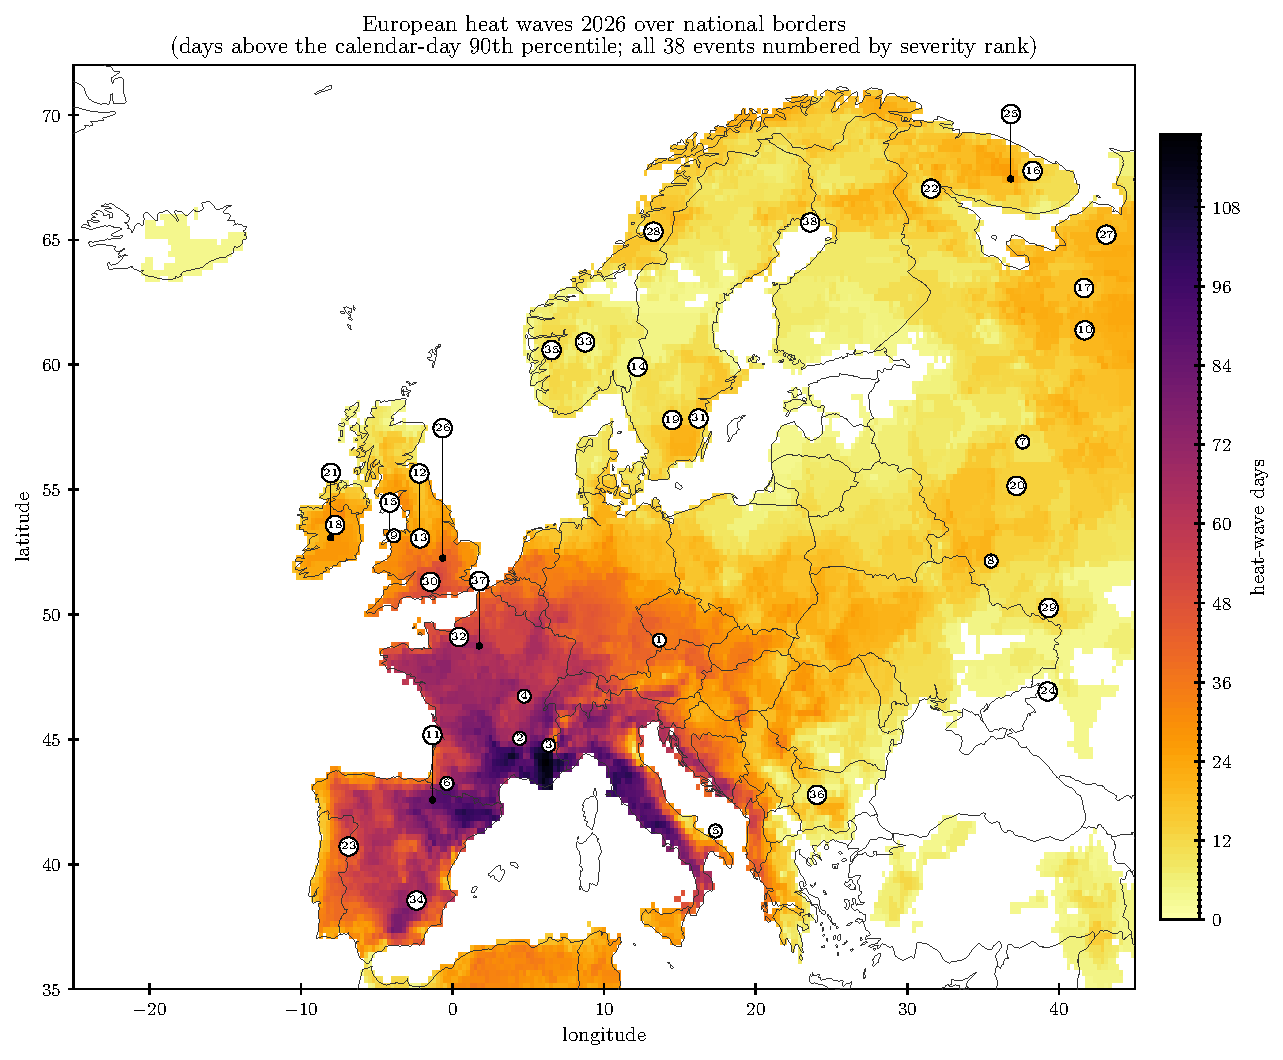
\includegraphics[width=\textwidth,height=0.75\textheight,keepaspectratio]{fig1}
  \caption{Number of days each land cell spent inside any of the
    \NEventsTwentySix{} events detected in 2026 with the reference
    configuration (section~\ref{sec:sensitivity}). Numbers mark event
    centroids and give the severity rank.}
  \label{fig:map}
\end{figure}

\begin{figure}[tbp]
  \centering
  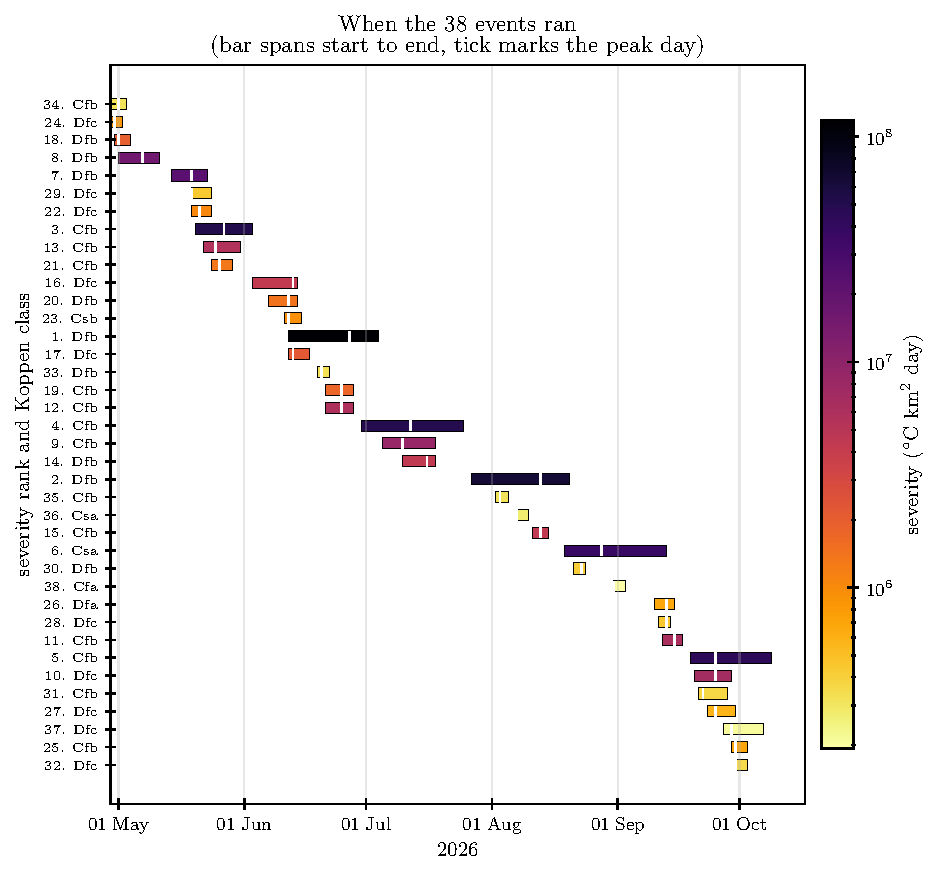
\includegraphics[width=\textwidth,height=0.75\textheight,keepaspectratio]{fig2}
  \caption{Duration of each 2026 event, ordered by start date and shaded by
    severity. The tick inside each bar marks the peak day. Labels give the
    severity rank and the modal K\"oppen-Geiger class.}
  \label{fig:timeline}
\end{figure}

\begin{figure}[tbp]
  \centering
  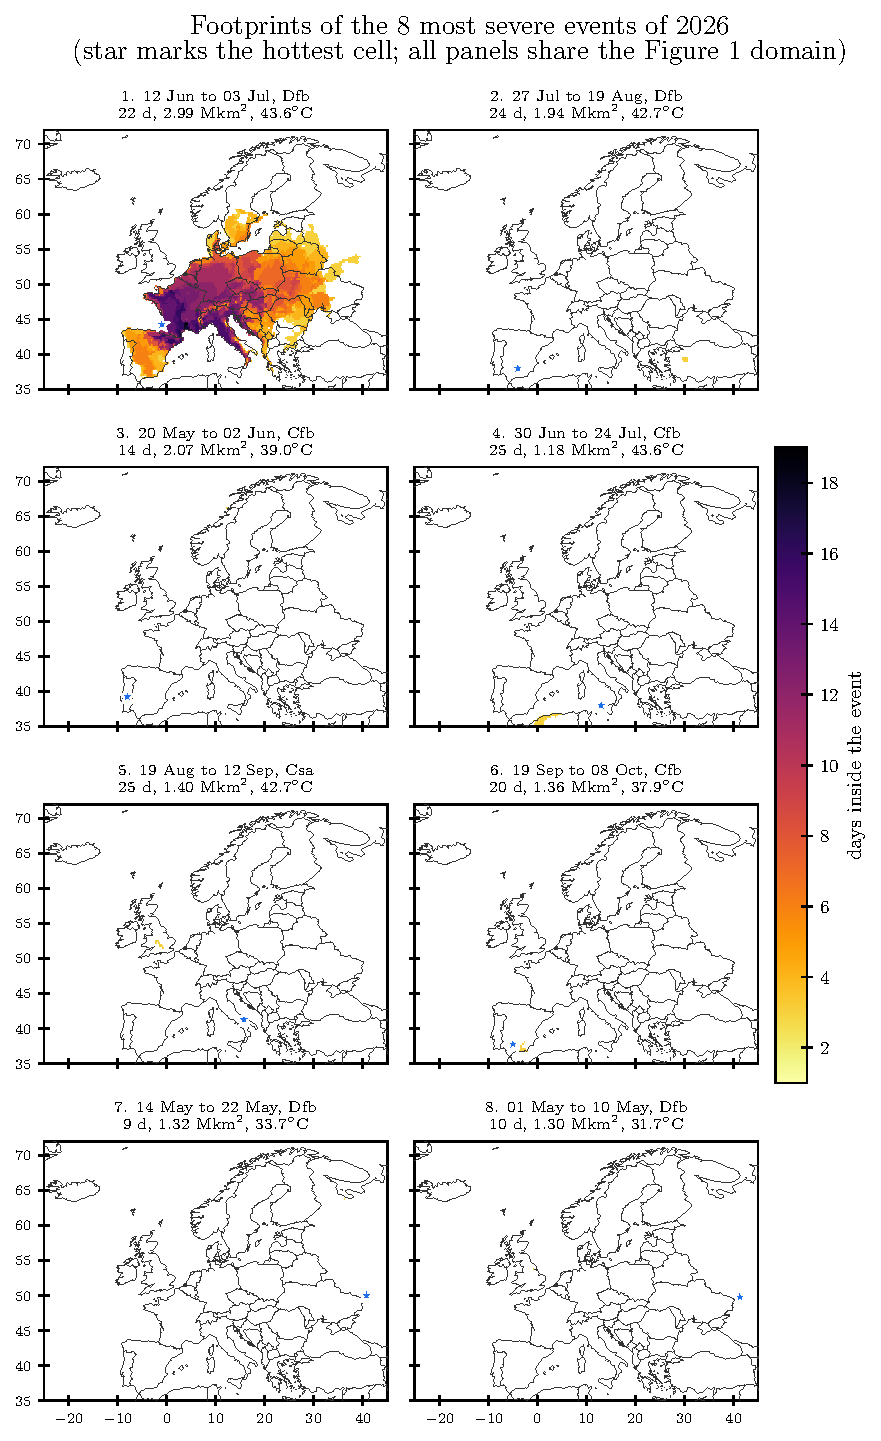
\includegraphics[width=\textwidth,height=0.75\textheight,keepaspectratio]{fig3}
  \caption{Footprints of the eight most severe events of 2026: the number
    of days each cell spent inside the event. The star marks the cell that
    recorded the event's highest daily maximum temperature.}
  \label{fig:footprints}
\end{figure}

\begin{figure}[tbp]
  \centering
  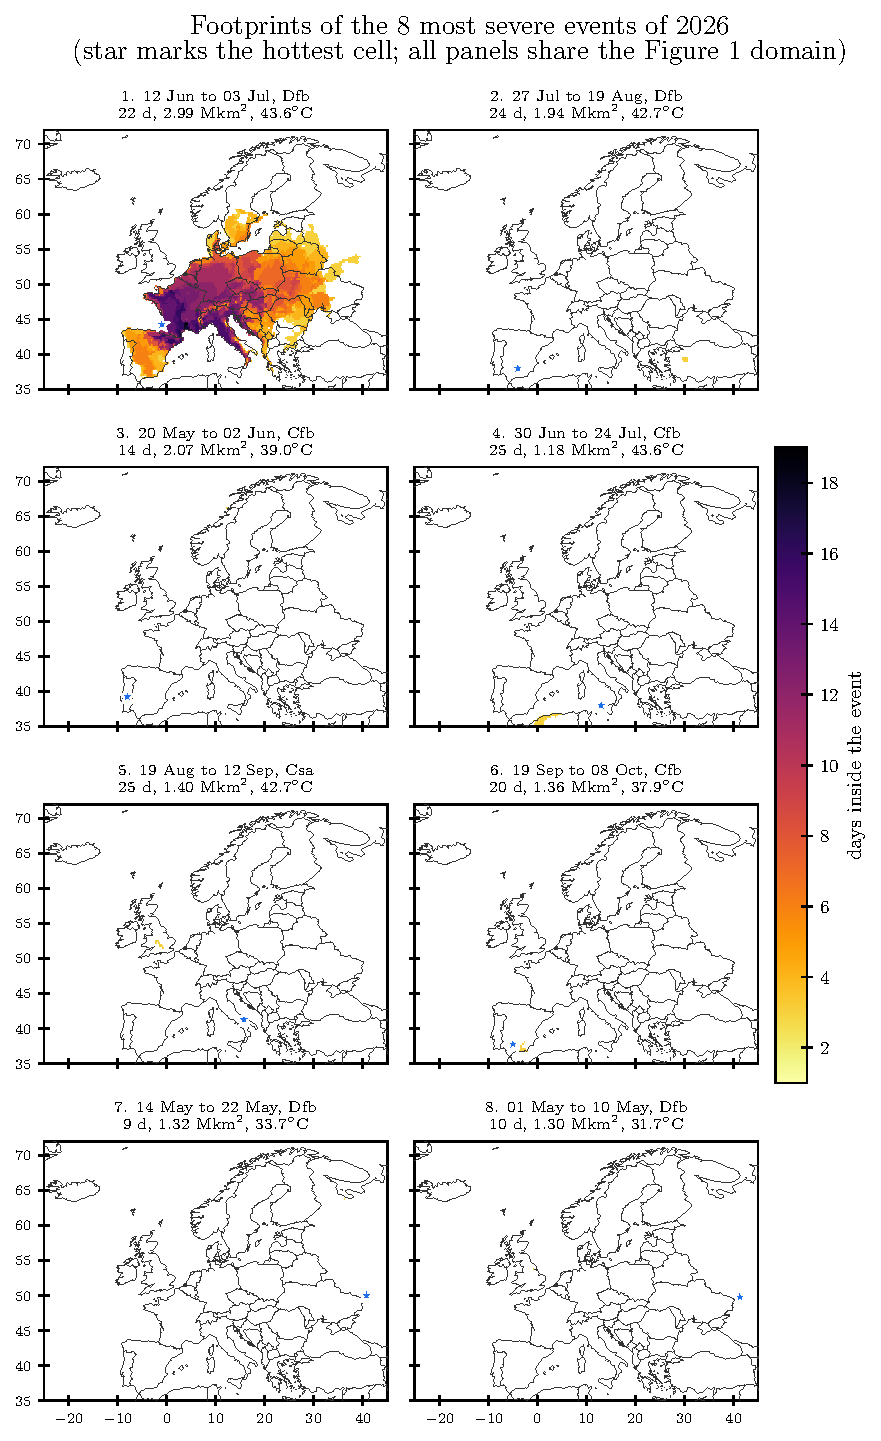
\includegraphics[width=\textwidth,height=0.75\textheight,keepaspectratio]{fig4}
  \caption{Change in severity rank of the six most severe reference events
    of each season under each configuration, defined as reference rank
    minus new rank, so that a positive value is a rise. Blank cells are
    unchanged. Column heads give $A_{\min}$, and the numbers beneath each
    panel give the total number of events detected. The blue outline joins
    reference events that a configuration detects as a single event.
    Events are matched by shared cell-days (section~\ref{sec:matching});
    summers inside 1991--2020 use a leave-one-out baseline.}
  \label{fig:sensitivity}
\end{figure}

\clearpage

\section{Discussion}
\label{sec:discussion}

%% TODO. Written third.

\section{Conclusions}
\label{sec:conclusions}

%% TODO.

\datastatement
%% TODO. AMS requires this section. It needs the Zenodo DOI for the deposited
%% catalogues, the ERA5 CDS citation, and the code repository.

%% PREVIEW: swap back to ametsocV6 once the AMS files are here.
\bibliographystyle{plainnat}
\bibliography{references}

\end{document}
